\section{Schnittstellen}

\subsection{Übersicht}
Da in diesem Projekt nur ein Mikrokontroller verwendet wird, halten sich die Hardwareschnittstellen in Grenzen.

\subsection{Hardwareschnittstellen}
Als Hardwareschnittstellen kommen lediglich Jumper-Kabel zum Einsatz, sowohl für die Datenübertragung als auch für die Versorgungsspannung. Dafür soll möglicherweise ein Kabelbaum zum Einsatz kommen. \\
\\
Wir führen hier auch noch die Motorentreiber auf. Sie nutzen ein PWM-Signal, durch welches sie die ihnen zur Verfügung gestellte 24V Spannung in unterschiedlicher Stärke an die Motoren weitergeben. 

\begin{figure}[H]
    \begin{center}
    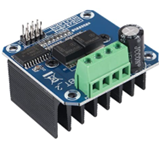
\includegraphics[width=4cm]{Hardware-Schnittstelle_PWM.png}
    \end{center}
    \caption{Motorentreiber}
\end{figure}

\subsection{Softwareschnittstellen}
Die Kommunikation zwischen den Sensoren und dem Arduino soll über das UART- und das I2C- Protokoll laufen. Das I2C-Protokoll benutzt die SCL- und SDA- Pins (A4- und A5 auf dem Arduino UNO), welche vom Kompass-Modul benutzt werden soll.\\
\\
Das GPS-Modul und das Bluetooth-Modul sollen über ein UART-Protokoll mit dem Arduino kommunizieren. Dafür sind alle Pins mit PWM-Funktion auf dem Arduino ausreichend. \\
\\
Die Motorentreiber erhalten ein 5V PWM-Signal welches sie in ihrer Ausgangsspannung, in unserem Fall 24V, weitergeben.
